\begin{block}{Experimental setup}
  \begin{figure}
    \begin{center}
      \includegraphics[width=.9\linewidth]{figures/experiment_big}
    \end{center}
    \label{Schematic of the experimental setup}
  \end{figure}
  $W$: output wedge, $BS$: beam splitter, $CTSDL$: cesium two-photon stabilized diode laser, $DG$: diffraction grating, $SLM$: spatial light modulator, $AOM$ acousto-optic modulator, $C$: mechanical chopper, $PMT$: photo-multiplier tube
  \begin{itemize}
  \item The repetition rate $f_{rep}$ is near integer fraction of the ground-state splitting (e.g. 1/100 $\approx$ 92 MHz )
  \item Repetition rate locked to 5th harmonic of synthetizer (that has 10~mHz stability)
  \item SLM band pass filter bandwith of $\approx$ 0.6 nm ($\approx$ 1 ps pulse length)
  \item Chopping frequency 500-1000 Hz
  \item Time-average input intensity 140$\mu$W with $<$1$\mu$W stability 
  \end{itemize}
\end{block}
